\section{溶液作製精度に関して}

溶液の作製精度の確認を行うため,0.95,1.00,1.05wt.\%のPAA溶液を作製した.それぞれの擬塑性流体に直径10mmの鋼球を落下させ,終端速度の変化,超音波照射による影響の変化の確認を行った.

\subsection{溶液の粘性特性に関して}
それぞれの溶液の特性を確認するため,粘度計を用いて粘度計測を行った.粘度計測を行った結果をFig.\ref{fig:95-105}に示す.比較のため,先行研究である岩室\cite{ref:8}とShiratori \it{et al}.\cite{ref:9}の計測結果も合わせて示す.濃度が薄いと粘度は低く,濃度が高いと粘度は高くなった.


\begin{figure}[ht]
    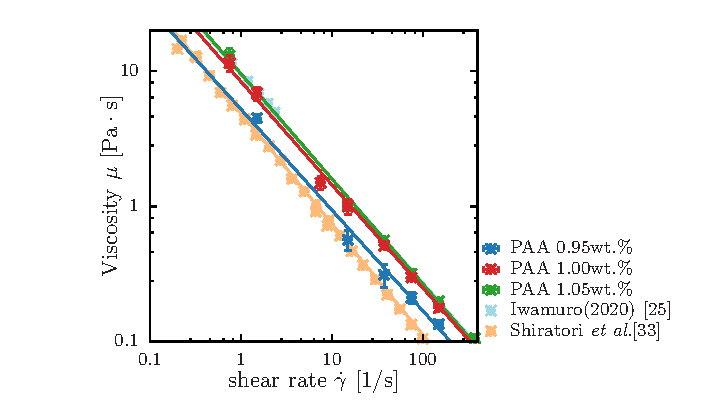
\includegraphics[width=1\textwidth]{X-Appendix/concentration/viscosity/viscosity.eps}
    \caption{Viscosity versus shear rate for PAA0.95,1.00,1.05wt.\%.}
    \label{fig:95-105}
\end{figure}

\subsection{溶液の作製精度による高速化への影響に関して}

ぞれぞれの質量濃度のPAA溶液に対し,落下球実験を行った.落下させた球は,鋼製の直径10mmの球である.
